\documentclass[twocolumn, a4paper]{ieicejsp}
\usepackage{newenum}
\usepackage{epsfig}

\title{{\bf 大会原稿執筆見本}
  {\normalsize \\ THE  WRITING  SAMPLE  FOR  THE  CONFERENCE}}
  \author{
    原田崇司$^1$ \\ Takashi  Harada \and
    田中賢$^1$ \\ Ken Tanaka \and
    三河賢治$^2$ \\ Kenji Mikawa
  }
  \affliate{
    (社)電子情報通信学会 集会事業部A$^1$ \\
    Conference Department, The Institute of Electronics, Information and Communication Engineers A
    \and
    (社)電子情報通信学会 集会事業部B$^2$ \\
    Conference Department, The Institute of Electronics, Information and Communication Engineers B
    \and
    Stanford University, Department of Information Science$^3$
}

\begin{document}
\maketitle
\section{まえがき}
原稿用紙はA4判白紙に原稿執筆見本に示す体裁に従って内容の記載・図表の添付を行います.従来の専用原稿用紙は使用する必要はございません.

講演論文集は,著者の原稿をそのまま原版とし,B5判(約86%に縮尺)により出版致します.「原稿」が不適当であると印刷に支障を来します.この説明書をよくお読みになった上で原稿をお書き下さい
\begin{table}[h]
\small
\caption{文字数の目安}
\begin{tabular}[t]{|c|c|}
\hline
  一般講演(A) & シンポジウム講演(B)\\
\hline
  1枚 / 1件         & 2枚 / 1件 \\
  44字×43行=1892字 & 44字×43行=1892字(1枚目) \\
                     & 44字×52行=2288字(2枚目) \\
\hline
\end{tabular}
\end{table}

\section{今回の相違点}
\begin{newenumerate}
\item Webによる講演申込 \\
講演申込受付期間内に、本会ホームページの投稿のページに開設する「大会講演参加申込方法」から登録して下さい.

正しく登録が受け付けられますと、「受付番号」・「登録済内容にアクセスするためのパスワード」などが登録受理票で表示されますので、申込者で必ずプリントアウトして保管し、論文の提出する際に原稿の左上にホチキス止で添付して下さい.

また、登録完了時点で入力項目の確認のために「受付回答メール」が申込者に送付されます.(必ず、内容の確認を行って下さい.)

講演申込受付期間内は受付番号とパスワードにより登録データの修正・取消が可能です.これに伴い、従来の専用講演申込書は不要となります.
\end{newenumerate}

\section{原稿作成要領}
\noindent※\underline{従来との相違点:学会所定の原稿用紙はありません.}
\begin{newenumerate}
\item A4判白紙に、原稿執筆見本に示す体裁に従って内容の記載・図表の添付を行います.

注意:提出された原稿は本会の「著作権」に関する事項が適用されます。ご了解の上,原稿を作成下さい

\item 講演原稿(	)は原寸で作成します。講演論文集にはB5判に縮小し,そのまま掲載されます.

\item 上下左右のマージンおよび講演番号スペースを確保します.マージンは上マージン30mm、左マージン18mm、カラム間マージン7mm、右マージン18mm、下マージン27mmを目安としてレイアウトに留意して下さい.

\item カラー写真は白黒になります.

\item 使用言語 日本語または英語.

\item 配置.
\begin{enumerate}
\item 表題,著者名,勤務先は原稿執筆見本に従い、記入して下さい.\\
英文の場合は,表題のみ英文で記入して下さい.
\item 本文は1段または2段に書いても差支えありません.
\end{enumerate}

\item 文字の大きさ.

表題,著者名,勤務先,本文の文字の大きさは,下記を大体の目安として下さい.
\begin{tabular}{lll}
表題 & 16ポイント = 5mm \\
著者名・勤務先・本文 & 10.5ポイント = 3mm
\end{tabular}
注意: 原稿は86%縮小(B5判)されますので文字の大きさを厳守して下さい.

\item 原稿には「登録受理票」のハードコピーを上に重ねて左上をホチキス止めし、折らずに封筒に入れ、学会事務局へご提出下さい.
\item \underline{提出期限は大会ホームページを確認してください。}
\item 提出後の差し替えはできません.
\item 原稿提出先
\begin{flushright}
〒105-0011 港区芝公園3-5-8 機械振興会館内 \\
(社) 電子情報通信学会 集会事業部大会係 \\
TEL: 03-3433-6691, FAX: 03-3433-6659
\begin{figure}[h]
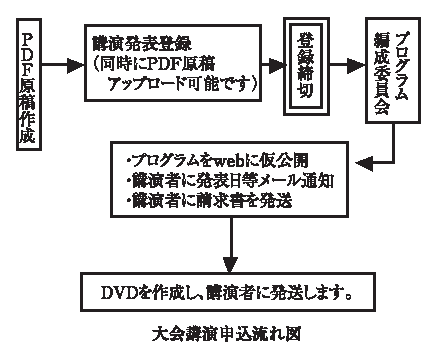
\epsfig{file=figure.eps}
\caption{大会講演申込流れ図}
\end{figure}
\end{flushright}
\end{newenumerate}
\end{document}
